\chapter{战术导弹动力学建模以及动力学特性分析}
\section{导弹动力学传递函数}
\section{导弹动力学8个特点}
\begin{enumerate}[1)]
    \item 直联项的影响
    \item 静稳定度$a_{24}$越大,固有频率越高
    \item 静稳定度越大,阻尼$\xi$越小
    \item 导弹极点并不会随着静稳定度变大而向左移,而是沿着平行于虚轴的直线远离实轴
    \item 静稳定度越大,导弹的响应速度越快。
    
    {\kaishu 此处注意区分理解“快速性”和“操纵性”:操纵性是导弹产生法向过载的难易程度,
    而阶跃响应的时间$t_r = \frac{\pi - arccos\xi_{\dot{m}}}{\omega_{m}\sqrt{1-\xi_{m}^2}}$
    可以描述导弹的“快速性”
    
    补充:《自动控制原理》
    
    一个欠阻尼二阶系统,其两个极点的复域如图\ref{exrem_point}所示,其中$\omega_d$为有阻尼自然震荡频率,$\omega_n$为无\dots:
    \begin{figure}[H]
        \centering
        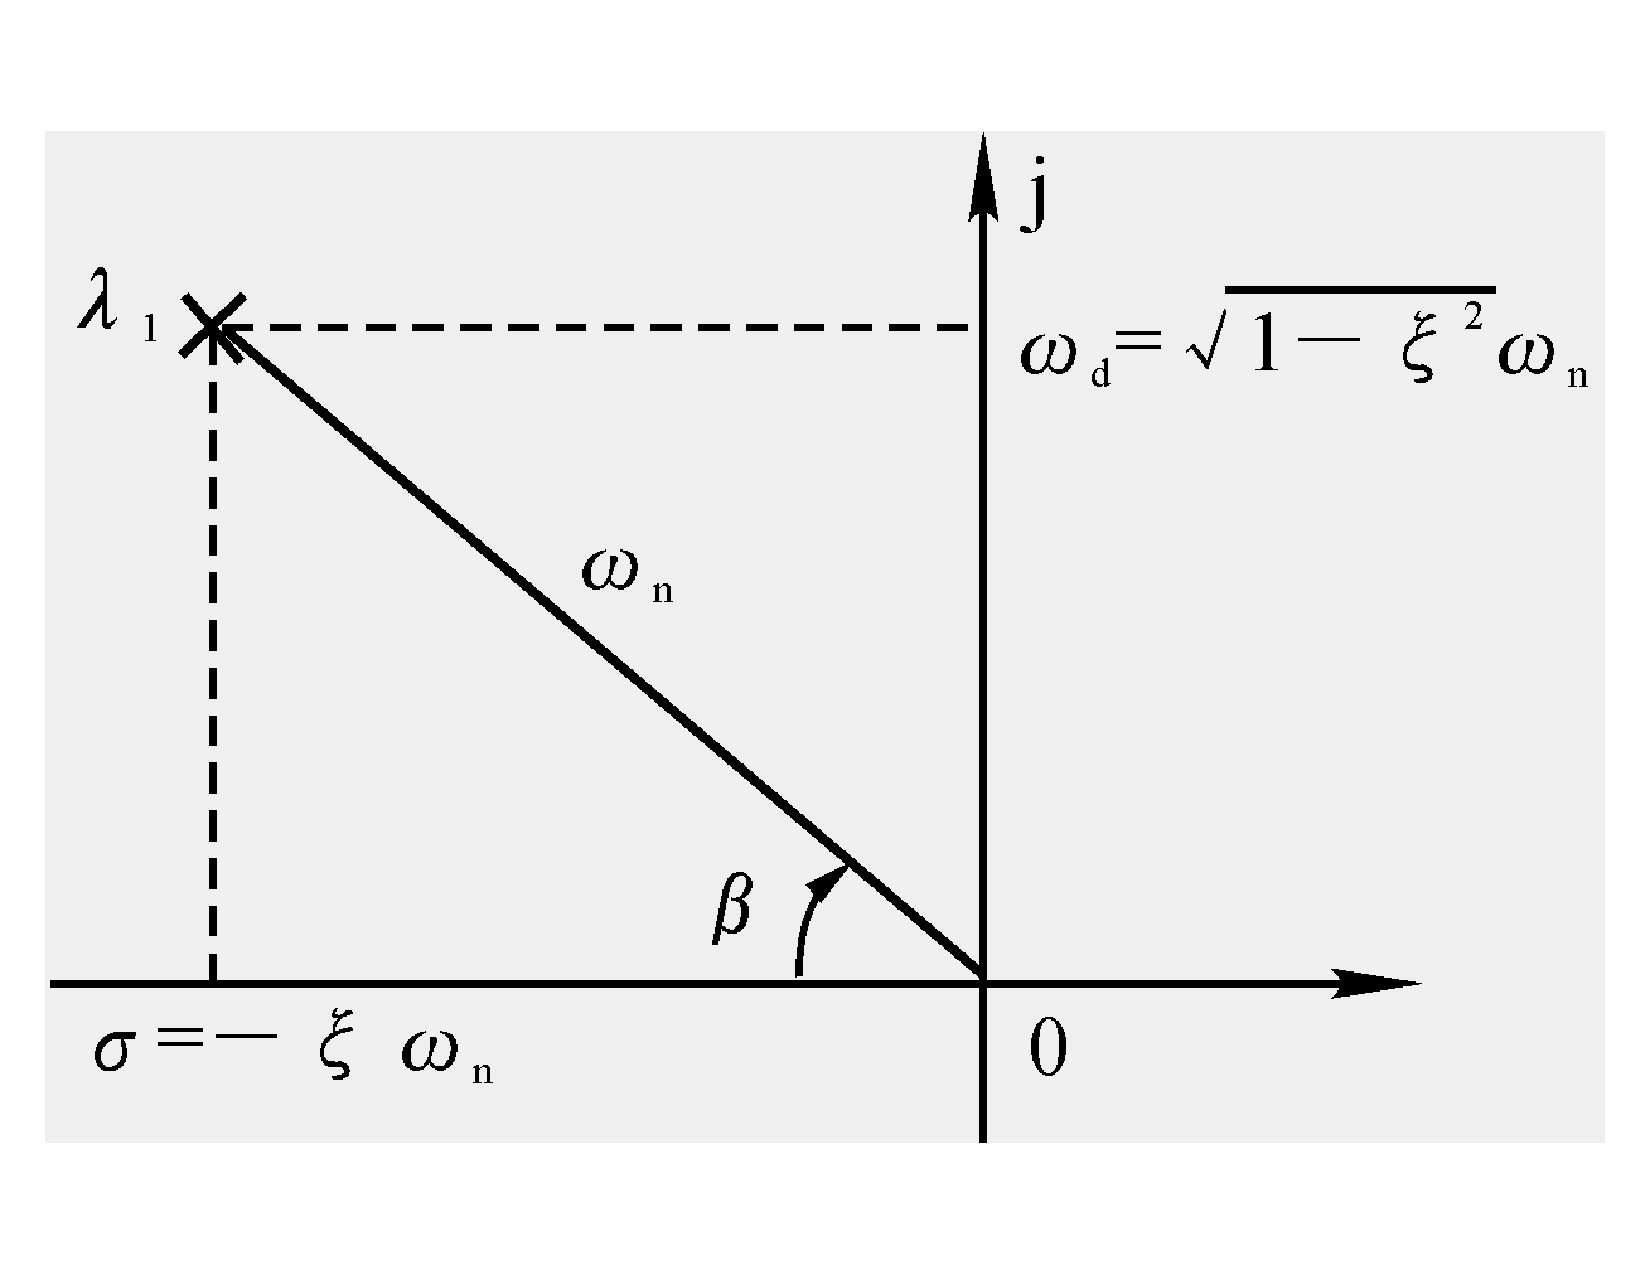
\includegraphics[scale = 0.35]{pictures/chapter8/2_order}
        \caption{二阶欠阻尼系统极点}
        \label{exrem_point}
    \end{figure}
    \begin{enumerate}[i]
        \item 阻尼比:$\xi = \cos\beta$ 
        \item 上升时间:$t_r = \frac{\pi-\beta}{\omega_d}$,其中$\beta = arccos\xi$
        \item 峰值时间:$t_p = \frac{\pi}{\omega_d}$
        \item 最大超调量:$\sigma\% = e^{-\pi\xi\sqrt{1-\xi^2}}\times100\%$
        \item 调节时间:当$\Delta = 0.5$时,$t_s\approx \frac{3}{\xi\omega_n}$;
                        当$\Delta = 0.3$时,$t_s\approx \frac{4}{\xi\omega_n}$;
    \end{enumerate}
    }
    \item 鸭式导弹和正常布局导弹的响应速度并无区别;鸭式导弹的稳态增益大于正常布局导弹,
    在0时刻的导弹的法向加速度,鸭式为正,正常式为负。(其实就是考虑直联项的影响)
    \item 静稳定的导弹考虑只短周期时,两个极点是在左半开平面,但长周期未必都在。
    \item 导弹动力学本身就是一个具有反馈的系统,“过载自动驾驶仪就是弹体动力学的自然延伸。”
\end{enumerate}
\section{状态空间表达式下的弹体动力学}
校正网络的实质是增加开环的零极点,使得根轨迹通过指定位置。
状态空间采用全状态反馈可以实现零极点的任意配置。
\subsection{状态空间}
纵向小扰动方程,俯仰角速度$\Delta\dot{\vartheta}=\Delta\omega_z$
\begin{equation*}
    \left[
        \begin{smallmatrix}
            \Delta\dot{V}\\
            \Delta\dot{\omega_z}\\
            \Delta\dot{\alpha}\\
            \Delta\dot{\vartheta}
        \end{smallmatrix}
    \right] = 
    \left[
    \begin{smallmatrix}
        a_{11} & 0 &a_{14}-a_{13} a_{13} \\
        a_{21}-a_{24}'a_{31} &a_{22}+a_{24}' &-a_{24}'a_{34}+a_{24}'a_{33}+a_{24} &-a_{24}'a_{33}\\
        -a_{31} &1 &-a_{34}+a_{33} &-a_{33}\\
        0 &1 &0 &0
    \end{smallmatrix}
    \right]
    \left[
    \begin{smallmatrix}
        \Delta{V}\\
        \Delta{\omega_z}\\
        \Delta{\alpha}\\
        \Delta{\vartheta}
    \end{smallmatrix}
    \right]+
    \left[
    \begin{smallmatrix}
        0\\
        a_{25}-a_{24}'a_{35}\\
        -a_{35}\\
        0
    \end{smallmatrix}
    \right]
    \Delta\delta_z
\end{equation*}

短周期运动的小扰动方程的状态向量可以是:
\begin{equation*}
    \left[
    \begin{smallmatrix}
        \vartheta \\
        \dot{\vartheta} \\
        \theta
    \end{smallmatrix}    
    \right]
    、
    \left[
    \begin{smallmatrix}
        \vartheta \\
        \dot{\vartheta} \\
        \alpha
    \end{smallmatrix}    
    \right]
    或者
    \left[
        \begin{smallmatrix}
            \alpha\\
            \vartheta \\
            \dot{\vartheta}
        \end{smallmatrix}    
        \right]
\end{equation*}


弹道倾角角速度以有其他的状态量以及输入唯一确定,不是状态变量。

忽略重力的影响$a_{33}=\frac{g\sin\theta}{V}$,可以得到用攻角以及俯仰角速度为状态变量短周期方程:
\begin{equation}
    \left[
        \begin{smallmatrix}
            \Delta\dot{\alpha}\\
            \Delta\dot{\dot{\vartheta}}
        \end{smallmatrix}
    \right] = 
    \left[
    \begin{smallmatrix}
        a_{33}-a_{34} &1\\
        a_{24} &a_{22}
    \end{smallmatrix}
    \right]
    \left[
    \begin{smallmatrix}
        \Delta{\alpha}\\
        \Delta{\dot{\vartheta}}
    \end{smallmatrix}
    \right]+
    \left[
    \begin{smallmatrix}
        -a_{35}\\
        a_{25}
    \end{smallmatrix}
    \right]
    \Delta\delta_z
    \label{simple_form}
\end{equation}

忽略舵面的力的影响$a_{35}=\frac{Y^{\delta_z}}{mV}$,
最终会得到法向过载以及攻角的关系式:$\alpha =\frac{f_y}{(a_{34}-a_{33})V}$
再将其带入公式\eqref{simple_form},得到以法向过载和俯仰角速度为状态变量的表达式:
见课本公式(8-57),这个形式下的状态空间表达式将在过载自动驾驶以设计时十分有用。
\section{导弹线性分式变换模型}
太难了,没写,考不考不知道。。